\documentclass[11pt]{article}

\usepackage[margin=2.5cm]{geometry}
\usepackage{graphicx}
\usepackage{booktabs}
\usepackage{siunitx}
\usepackage{hyperref}
\usepackage{amsmath}

% Auto-generated by `python -m fisicai.writeup` -- do not edit by hand.
\newcommand{\NEventsTotal}{83343}
\newcommand{\NEventsTwoMuons}{11983}
\newcommand{\NEventsOppositeCharge}{10420}
\newcommand{\NEventsMassWindow}{8589}
\newcommand{\BinWidthGev}{0.5}
\newcommand{\MassWindowLo}{60}
\newcommand{\MassWindowHi}{120}
\newcommand{\FitLo}{85}
\newcommand{\FitHi}{97}
\newcommand{\PtMin}{20}
\newcommand{\EtaMax}{2.4}
\newcommand{\MZPeak}{91.002}
\newcommand{\MZPeakStat}{0.041}
\newcommand{\MZPeakSystRange}{0.122}
\newcommand{\SigmaRes}{1.19}
\newcommand{\SigmaResStat}{0.07}
\newcommand{\NSigFit}{6446}
\newcommand{\NSigFitStat}{191}
\newcommand{\NBkgFit}{978}
\newcommand{\ChiTwo}{25.1}
\newcommand{\Ndf}{19}
\newcommand{\ChiTwoNdf}{1.32}
\newcommand{\GammaZPdg}{2.4955}
\newcommand{\MZPdg}{91.1880}
\newcommand{\MZPdgErr}{0.0020}
\newcommand{\PeakMinusPdgMev}{-186}
\newcommand{\PeakMinusPdgPermille}{2.0}


\title{Analysis note: position of the $Z\to\mu^{+}\mu^{-}$ resonance peak\\
in the CMS 2012 \texttt{DoubleMuParked} Open Data skim}
\author{fisicai analysis bundle}
\date{July 19, 2026}

\begin{document}
\maketitle

\begin{abstract}
The dimuon invariant-mass spectrum is reconstructed from a skim of the CMS
2012 \texttt{DoubleMuParked} Open Data sample. Events with exactly two
opposite-charge muons with $p_{\mathrm{T}} > \PtMin\,\text{GeV}$ and
$|\eta| < \EtaMax$ are selected, and the $Z$ resonance peak position is
extracted with a binned $\chi^{2}$ fit of a Voigtian signal plus an
exponential background in the
$\FitLo$--$\FitHi\,\text{GeV}$ mass range. The fitted peak position is
$m_{\mu\mu}^{\text{peak}} = \MZPeak \pm \MZPeakStat\,(\text{stat.}) \pm
\MZPeakSystRange\,(\text{fit range})\,\text{GeV}$; the difference with
respect to the PDG world-average $Z$ mass is
$\PeakMinusPdgMev\,\text{MeV}$ ($\PeakMinusPdgPermille$ per mille). No muon momentum-scale or final-state-radiation
corrections are applied, so the result is a peak-position determination, not
a $Z$ mass measurement.
\end{abstract}

\section{Introduction}

The $Z$ boson decaying to two muons produces one of the cleanest signatures
at a hadron collider: a narrow resonance at
$m_{Z} = \MZPdg \pm \MZPdgErr\,\text{GeV}$ \cite{ParticleDataGroup:2024cfk}
on top of a small, smoothly falling Drell--Yan and misreconstruction
background. This note documents a self-contained determination of the dimuon
peak position in real proton--proton collision data recorded by the CMS
detector \cite{CMS:2008xjf} in 2012 at $\sqrt{s} = 8\,\text{TeV}$ and
released through the CERN Open Data portal
\cite{Lassila-Perini:2021xzn}. The goal is a reproducible analysis bundle:
every number quoted here is generated by \texttt{analysis.py} and imported
into this document as a macro, so the note and the code cannot drift apart.

\section{Data}

The input is \texttt{zmumu\_skim.root}, a skim of the CMS 2012
\texttt{DoubleMuParked} primary dataset published on the CERN Open Data
portal (\url{https://opendata.cern.ch}) and converted to a flat
NanoAOD-like format with the CMS \texttt{AOD2NanoAODOutreachTool}
\cite{Lassila-Perini:2021xzn}. The skim contains \NEventsTotal{} events
with jagged per-muon branches \texttt{Muon\_pt}, \texttt{Muon\_eta},
\texttt{Muon\_phi}, \texttt{Muon\_mass}, and \texttt{Muon\_charge}
(momenta and masses in GeV). Only raw event counts are used throughout: no
luminosity normalization, pile-up reweighting, or trigger-efficiency
correction is applied, none of which affect the position of the resonance
peak.

\section{Event selection}

Muons are required to have $p_{\mathrm{T}} > \PtMin\,\text{GeV}$ and
$|\eta| < \EtaMax$, matching the muon-system acceptance
\cite{CMS:2008xjf}. Events must contain exactly two such muons with
opposite charge. The dimuon invariant mass is computed from the four-momentum
sum of the two muons, and the spectrum is analyzed in the
$\MassWindowLo \leq m_{\mu\mu} < \MassWindowHi\,\text{GeV}$ window. The
cutflow is given in Table~\ref{tab:cutflow}.

\begin{table}[htbp]
  \centering
  \caption{Event selection cutflow. Raw (unweighted) event counts.}
  \label{tab:cutflow}
  \begin{tabular}{lr}
    \toprule
    Selection & Events \\
    \midrule
    All events in skim & \NEventsTotal \\
    Exactly two muons, $p_{\mathrm{T}} > \PtMin\,\text{GeV}$, $|\eta| < \EtaMax$ & \NEventsTwoMuons \\
    Opposite charge & \NEventsOppositeCharge \\
    $\MassWindowLo \leq m_{\mu\mu} < \MassWindowHi\,\text{GeV}$ & \NEventsMassWindow \\
    \bottomrule
  \end{tabular}
\end{table}

\section{Method}

The selected masses are histogrammed in $\BinWidthGev\,\text{GeV}$ bins. The
spectrum is fitted by minimizing a $\chi^{2}$ with Poisson bin
uncertainties, using the model
\begin{equation}
  \frac{dN}{dm} \;=\; n_{\text{sig}}\,
  V\!\left(m - \mu;\, \sigma,\, \Gamma_{Z}/2\right)
  \;+\; n_{\text{bkg}}\, f_{\text{bkg}}(m),
\end{equation}
where $V$ is a Voigtian --- a relativistic-width Breit--Wigner convolved
with a Gaussian resolution of width $\sigma$ --- and $f_{\text{bkg}}$ is a
falling exponential normalized over the fit range, so that
$n_{\text{sig}}$ and $n_{\text{bkg}}$ are yields in that range. The
Breit--Wigner width is fixed to the PDG $Z$ width
$\Gamma_{Z} = \GammaZPdg\,\text{GeV}$ \cite{ParticleDataGroup:2024cfk};
the Gaussian $\sigma$ absorbs the detector resolution. The nominal fit uses
the $\FitLo$--$\FitHi\,\text{GeV}$ core of the peak, excluding the low-mass
tail populated by final-state radiation (FSR), which the symmetric Voigtian
does not model.

The sensitivity of the peak position to this choice is assessed by repeating
the fit with three alternative ranges ($80$--$100$, $83$--$99$, and
$86$--$96\,\text{GeV}$, as defined in \texttt{analysis.py}); the largest
absolute shift of the fitted peak is taken as a fit-range systematic
uncertainty.

\section{Results}

The nominal fit converges with
$\chi^{2}/\text{ndf} = \ChiTwo/\Ndf = \ChiTwoNdf$ and yields
\begin{equation}
  m_{\mu\mu}^{\text{peak}} \;=\;
  \MZPeak \;\pm\; \MZPeakStat\,(\text{stat.})
  \;\pm\; \MZPeakSystRange\,(\text{fit range})\;\text{GeV},
\end{equation}
with a Gaussian resolution
$\sigma = \SigmaRes \pm \SigmaResStat\,\text{GeV}$ and fitted yields of
$\NSigFit \pm \NSigFitStat$ signal and $\NBkgFit$ background events in the
fit range. The spectrum and fit are shown in
Figure~\ref{fig:dimuon_mass}.

\begin{figure}[htbp]
  \centering
  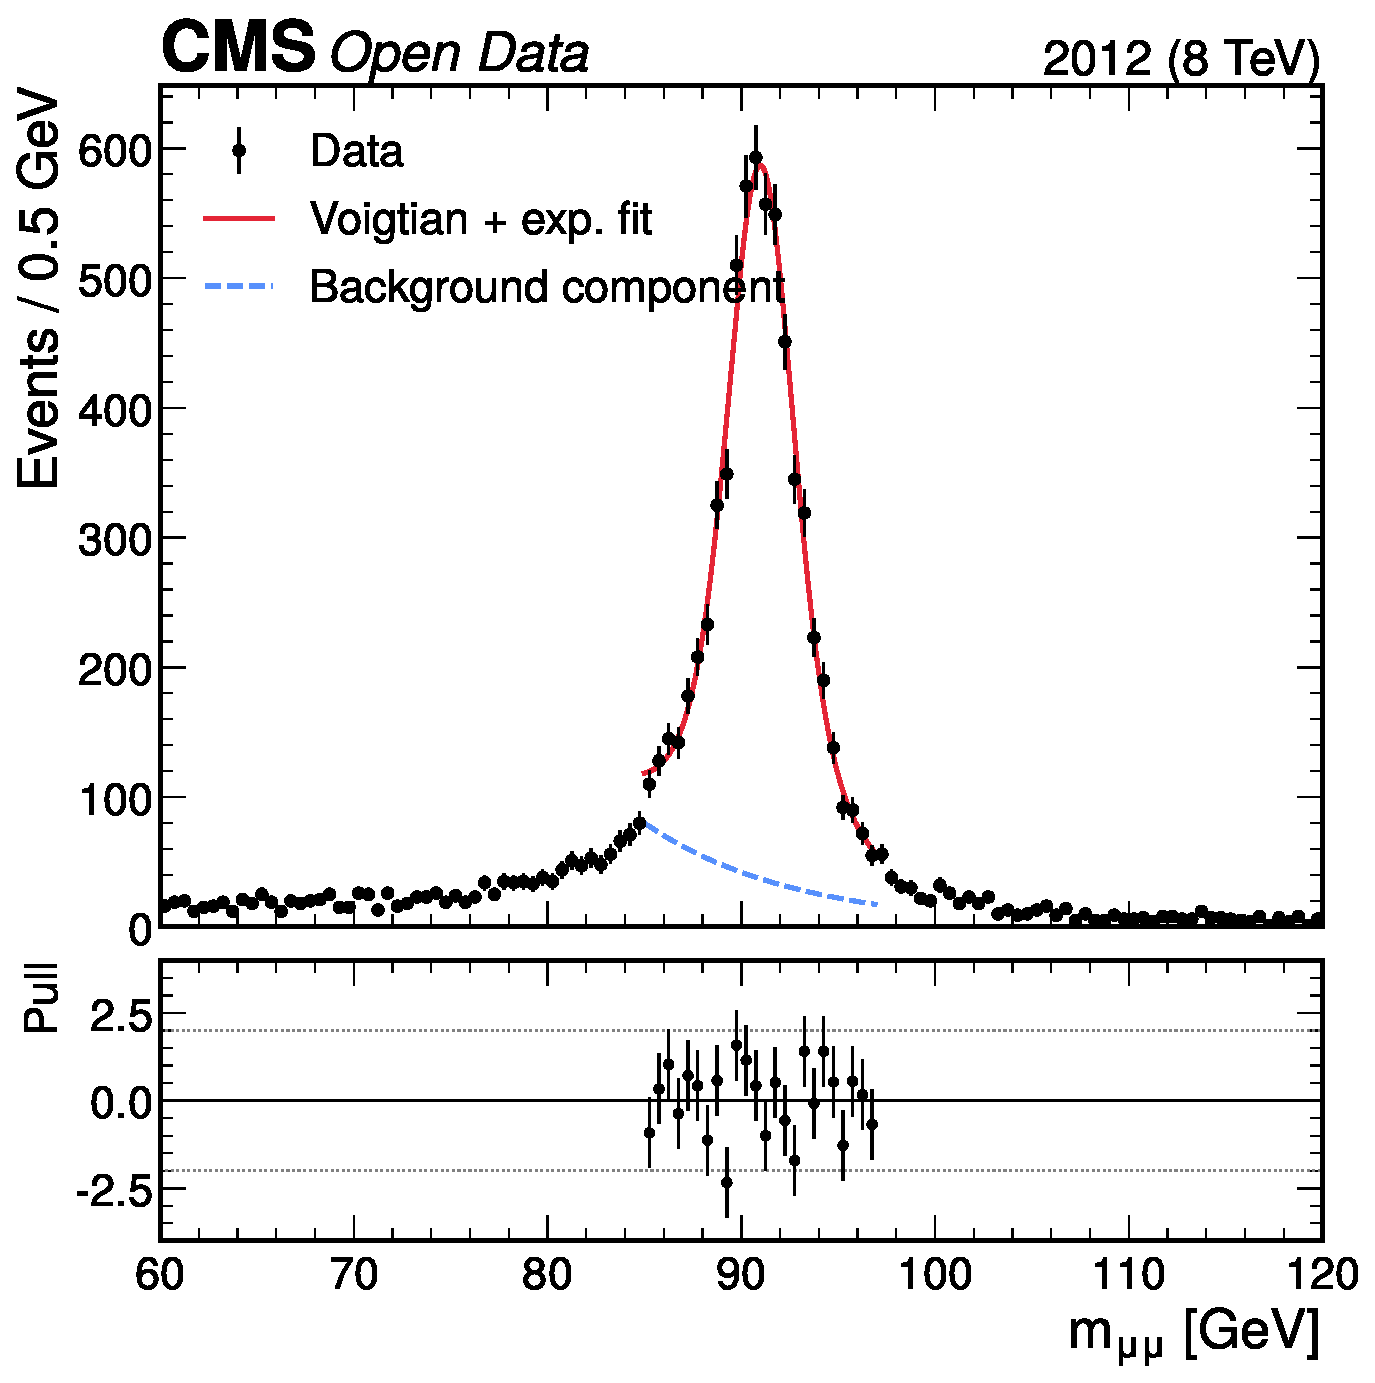
\includegraphics[width=0.78\textwidth]{../figures/dimuon_mass.pdf}
  \caption{Dimuon invariant-mass spectrum after the full selection
    (points), with the Voigtian-plus-exponential fit in the
    $\FitLo$--$\FitHi\,\text{GeV}$ range (solid line) and its background
    component (dashed line). The dotted vertical line marks the fitted peak
    position.}
  \label{fig:dimuon_mass}
\end{figure}

Compared with the PDG world average
$m_{Z} = \MZPdg \pm \MZPdgErr\,\text{GeV}$
\cite{ParticleDataGroup:2024cfk}, the difference
$m_{\mu\mu}^{\text{peak}} - m_{Z}$ is $\PeakMinusPdgMev\,\text{MeV}$, a
relative difference of $\PeakMinusPdgPermille$ per mille. This difference
is comparable to the
combined quoted uncertainties, and its sign is the one expected from the
two dominant effects deliberately left uncorrected here: unrecovered FSR
photons, which shift the reconstructed peak below the pole, and the muon
momentum scale, which is not calibrated in this open-data skim.

\paragraph{Uncertainties not evaluated.}
Only the statistical uncertainty from the fit and the fit-range variation
are quantified. Not evaluated are: the muon momentum-scale and resolution
calibration (the dominant systematic in a real $Z$ mass measurement), the
modeling of FSR, the choice of signal parameterization (a symmetric
Voigtian, with $\Gamma_{Z}$ fixed) and of the background shape, and any
alignment- or charge-dependent momentum biases. For this reason the result
is presented as a determination of the reconstructed peak position, and no
claim of a competitive $Z$ mass measurement is made.

\section{Conclusion}

The $Z\to\mu^{+}\mu^{-}$ resonance is clearly reconstructed in the CMS 2012
\texttt{DoubleMuParked} Open Data skim, with \NEventsMassWindow{} selected
events in the $\MassWindowLo$--$\MassWindowHi\,\text{GeV}$ window. The
fitted peak position of
$\MZPeak \pm \MZPeakStat\,(\text{stat.}) \pm
\MZPeakSystRange\,(\text{fit range})\,\text{GeV}$ agrees with the PDG $Z$
mass at the per-mille level, demonstrating that the public skim, the
selection, and the fitting chain are sound. The full analysis is
reproducible from \texttt{analysis.py} as described in the bundle
\texttt{README}.

\bibliographystyle{unsrt}
\bibliography{references}

\end{document}
